
\documentclass{standalone}
\usepackage{tikz}
\usetikzlibrary{arrows.meta, positioning}
\begin{document}
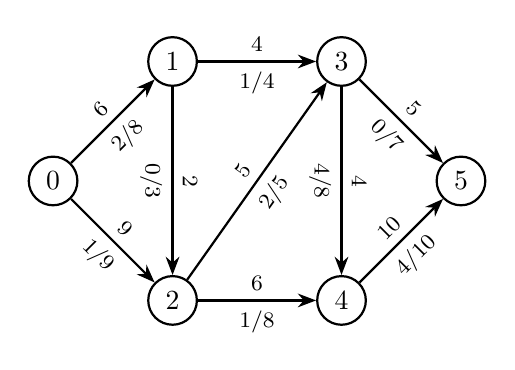
\begin{tikzpicture}[
		node distance= {15mm},
		thick,
		main/.style= {
				draw,
				circle
			},
		myarrow/.style= {
				-Stealth
			}
	]

	\node[main](0) {$0$};
	\node[main] (1) [above right = of 0] {$1$};
	\node[main] (2) [below right = of 0] {$2$};
	\node[main] (3) [right = of 1] {$3$};
	\node[main] (4) [right = of 2] {$4$};
	\node[main] (5) [below right = of 3] {$5$};
	\draw[myarrow] (0) to node[font =\footnotesize, sloped, midway, below] {2/8} node[font =\footnotesize, sloped, midway, above] {6} (1);
	\draw[myarrow] (0) to node[font =\footnotesize, sloped, midway, below] {1/9} node[font =\footnotesize, sloped, midway, above] {9} (2);
	\draw[myarrow] (1) to node[font =\footnotesize, sloped, midway, below] {1/4} node[font =\footnotesize, sloped, midway, above] {4} (3);
	\draw[myarrow] (1) to node[font =\footnotesize, sloped, midway, below] {0/3} node[font =\footnotesize, sloped, midway, above] {2} (2);
	\draw[myarrow] (2) to node[font =\footnotesize, sloped, midway, below] {2/5} node[font =\footnotesize, sloped, midway, above] {5} (3);
	\draw[myarrow] (2) to node[font =\footnotesize, sloped, midway, below] {1/8} node[font =\footnotesize, sloped, midway, above] {6} (4);
	\draw[myarrow] (3) to node[font =\footnotesize, sloped, midway, below] {4/8} node[font =\footnotesize, sloped, midway, above] {4} (4);
	\draw[myarrow] (3) to node[font =\footnotesize, sloped, midway, below] {0/7} node[font =\footnotesize, sloped, midway, above] {5} (5);
	\draw[myarrow] (4) to node[font =\footnotesize, sloped, midway, below] {4/10} node[font =\footnotesize, sloped, midway, above] {10} (5);
\end{tikzpicture}
\end{document}
